\section{Data assimilation}

\subsection{Intro}
\noindent Data assimilation is nowadays widely used to make predictions in complex systems, for example in weather forecasting or ocean prediction. Data assimilation is a method that combines observations with the output of a model to improve a prediction. 
The main idea is to combine information from our model and from observations, in order to have a more reliable analysis. Sometimes what you are trying to improve in your model may not be in the same space as what you observe this is something that you need to consider while doing your assimilation. It is also important to control our output, it is up to us to decide which input is responsible for the error in our output. This means that there will be uncertainties coming from the model or from the observations, these uncertainties coming from our input will also translate into uncertainties in our output.
At the end of this data assimilation we will have obtained an output which will be an estimate of the unknown quantity called the state variables.
The best estimate is searched for as a linear combination of the background estimate and the observations:

$$x^a=Lx^b+Ky^0$$


\noindent Data assimilation methods are often split into two families: variational methods and statistical methods.
The first method, called variational methods, consists in minimizing a cost function with the least squares approach. 
\subsection{statistical approach}
\subsubsection{Kalman filter}
The Kalman filter method consists in looking for $x^a$ an analysis, this analysis will be a linear combination of what we already know, our model and our observations.
To explain this method let's consider that we observe a single quantity, an estimation of a scalar quantity at a point in space.For example we are observing the temperature in the middle of the room, and the model also simulate the temperature in the middle of the room.  We will then have :
$$x^a=x^b+K(y-x^b)$$
with $x^a$ the analysis, $x^b$ the background or model, and $y$ the observation. 
We suppose that the true state $x^t$ exists so:
$$x^a-x^t+K(y-x^t-x^b+x^t)$$
let's define the errors:
$$\begin{aligned}
&\epsilon^a=x^a-x^t \\
&\epsilon^b=x^b-x^t \\
&\epsilon^y=y-x^t \\
\end{aligned}$$
So we will have:
$$\epsilon^a=\epsilon^b+K(\epsilon^y-\epsilon^b)$$
If we have many realisation of these error, then we will have:
$$<\epsilon^a>=<\epsilon^b>+K(<\epsilon^y>-<\epsilon^b>)$$
We want to have the analysis error variance as low as possible .So we want to minimize $<(\epsilon^a)^2>$ with respect to $K$ ,this will give us:
$$<(\epsilon^a)^2>=<(\epsilon^b)^2>+K^2<(\epsilon^y-\epsilon^b)^2>+2K<\epsilon^b(\epsilon^y-\epsilon^b)^2>$$
$$2k<(\epsilon^y)^2+(\epsilon^b)^2>-2<(\epsilon^b)^2>=0$$
\noindent We assume that the errors in the background and observation are uncorrelated.
$$K=\frac{<(\epsilon^b)^2>}{<(\epsilon^b)^2>+<(\epsilon^y)^2>} \Rightarrow K=\frac{(\sigma^b)^2}{(\sigma^b)^2+(\sigma^y)^2} $$
where $(\sigma^y)^2$ is the observation error variance and $(\sigma^b)^2$ is the background or model error variance.
\newline\noindent If we have $(\sigma^y)^2=0$, $K=1$ and $x^a=y$  this means that the observation are perfect.
\newline\noindent And if $(\sigma^b)^2=0$, $K=0$ and $x^a=x^b$ this is equivalent to ignoring the observations.
\vspace*{5mm}
\newline Now that we have explained the method for solving $x^a$ let's try to generalize our formula.

$$\left\{\begin{aligned}
		&x^a=(I-KH)x^b+Ky^0=x^b+K(y^0-H(x^b)) \\
        &K=BH^T(HBH^T+R)^{-1} \\
	\end{aligned}\right.$$
With $K$ the gain or weight matrix, $(y^0-H(x^b))$ the innovation and $H$ the linear model of the observations.
This formulation is called the Best Linear Unbiased Estimator(BLUE) or least squares analysis.
The principle of the Kalman filter is based on this formulation. Here is a small figure which illustrates the Kalman filter.
\vspace*{5mm}
\begin{center}
		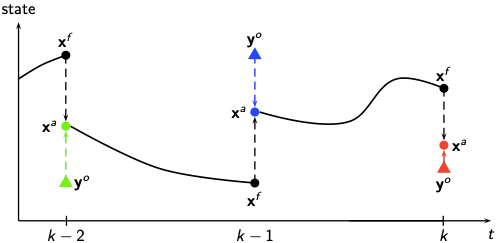
\includegraphics[width=0.8\textwidth]{"images/schema_kalman_filter.png"}
	\end{center}
The general idea consists in estimating the state at time $k$ from an estimate at time $k-1$ and measurements at time $k$.
We do the estimation in two steps:
\begin{enumerate}[label=\textbullet]
		\item Prediction of the state from the evolution model
		\item Correction of the prediction from the measurements
	\end{enumerate}

\subsubsection{Kalman filter algorithm}
For the notations we will use:

\noindent Vector:
 \begin{enumerate}[label=\textbullet]
		\item $k$ time index
		\item $x_{k}^{f}$ forecast state (background), forecast error covariance matrix $P_{k}^{f}$
		\item $x_{k}^{a}$ analyzed state (result of the assimilation process), analysis error covariance matrix $P_{k}^{a}$
	\end{enumerate}
\noindent Operators:
    \begin{enumerate}[label=\textbullet]
		\item model operator $x_{k+1}^{t} = M_{k,k+1}(x_{k}^{t})+ \eta
		_{k,k+1}$, model error $\eta
		_{k,k+1}$, covariance matrix $Q_k$
		\item observation operator $y_k^o = H_k (x^t ) + \epsilon_k^0$ , observation error $\epsilon^0$, covariance matrix $R_k$
	\end{enumerate}
\noindent The hypotheses necessary for the application of the Kalman filter are:
    \begin{enumerate}[label=\textbullet]
		\item Model and observations operators $M_{k,k+1}$ and $H_k$ are linear.
		\item Errors are unbiased, Gaussian, independent and white in time.
	\end{enumerate}
So finally we obtain the Kalman filter algorithm.
\begin{enumerate}[label=(\roman*)]
\item Initialization: $x_0^f$ and $P_0^f$ are given, equal to $x^b$ and $B$
\item BLUE:
$$\begin{aligned} &K_k=(H_kP_k^f)^T[H_k(H_kP_k^f)^T+R_k]^{-1} \\
&x_k^a=x_k^f+K_k(y_k^0-H_kx_k^f) \\
&P_k^a=(I-K_kH_k)P_k^f \\
\end{aligned}$$
\item Forecast step:
$$\begin{aligned} 
&x_{k+1}^f=M_{k,k+1}x_k^a \\
&P_{k+1}^f=M_{k,k+1}P_k^aM_{k,k+1}^T+Q_k\\
\end{aligned}$$
\end{enumerate}



\subsection{Variational approach}
\subsubsection{Minimizing a cost function}
\noindent In the previous part we have seen that there is a method called kalman filter which purpose is to make prediction with a model and observations, but there is also other method to make data assimilation like the variational assimilation, which solves the analysis problem through an optimisation (minimisation of a cost-function). This allows to solve the global problem in one go, and it is now widely used in the meteorological community. So variational data assimilation methods lead to the minimization of a cost function involving quadratic forms based on the both the background and observation covariance matrices. When the observation operator is linear the formulation of the cost function leads to the best the Best Linear Unbiased Estimation.An alternative way to define the analysis is to consider it as the maximum of the a posteriori p.d.f of the state given the observation and the background:
$$x^a=\arg\max_{x}p(x|y ~ and ~ x^b)$$
Using bayesian appreach $p(x|y)~\alpha~ p(y|x)p(x)$ we can simplify our probability by:
$$p(x|y ~ and ~ x^b)=\frac{p(y ~ and ~ x^b| x)p(x)}{p(y ~ and ~ x^b)}$$
We assume that observation and background errors are uncorrelated so we will have then:
$$(x|y ~ and ~ x^b)=p(y|x)p(x^b|x)$$
So we can define the cost function as:
$$J(x)=-log(p(y|x)p(x^b|x)+cst \\
=-log(p(y|x))-log(p(x^b|x))+cst$$
We can find the analysis by solving a minimization problem:
$$x^a=\arg\max_{x}J(x)$$
We assume that p.d.f are gaussien.
$$p(x^b|x)=(2\pi)^{-n/2}|B|^{-1/2}\exp({-\frac{1}{2}(x-x^b})^TB^{-1}(x-x^b))$$
$$p(y|x)=(2\pi)^{-m/2}|R|^{-1/2}\exp({-\frac{1}{2}(y-H(x)})^TR^{-1}(y-H(x)))$$
Which will lead us to:
$$J(x)=\frac{1}{2}(x^b-x)^TB^{-1}(x^b-x)+\frac{1}{2}(y-H(x))^TR^{-1}(y-H(x))$$
This is called the cost function of 3D-Var Approach.
\subsubsection{Generalisation of the 3D-Var Approach}
\noindent Let's go back to the notations:
\noindent Vector:
 \begin{enumerate}[label=\textbullet]
		\item $x$ state vector or input parameters
		\item $x^{b}$ background state (a priori information), background  error $\epsilon^b=x^b-x^t$ covariance matrix $B$
		\item $x^{a}$ analyzed state (result of the assimilation process)
		\item $y^0$ observation vector
	\end{enumerate}
\noindent Operators:
    \begin{enumerate}[label=\textbullet]
		\item model operator $x_{k}^{t} = M_{k,k-1}(x_{k-1}^{t})=M_{0 \rightarrow k}(x_0^t)$
		\item observation operator $y^0 = H (x^t) + \epsilon^0$, $y_k^0 = H_k(x^t) + \epsilon_k^0$ observation error $\epsilon_k^0$, covariance matrix $R_k$
	\end{enumerate}
\noindent Variational approach of BLUE consists in finding $x^a=\arg\max_{x}J$:
$$\begin{aligned}
J(x)&=\frac{1}{2}(x^b-x)^TB^{-1}(x^b-x)+\frac{1}{2}(y-H(x))^TR^{-1}(y-H(x)) \\
&=\frac{1}{2}\|x-x^b\|_B^2+\frac{1}{2}\|H(x)-y^0\|_R^2
\end{aligned}$$
If the problem is time-dependant, and the unknown x is the initial state vector:
$$\begin{aligned}
J(x)&=\frac{1}{2}\|x-x^b\|_B^2+\frac{1}{2}\|H_k(x)-y_k^0\|_{R_{k}}^2 \\
&=\frac{1}{2}\|x-x^b\|_B^2+\frac{1}{2}\|H_k(M_{0 \rightarrow k}(x))-y_k^0\|_{R_{k}}^2
\end{aligned}$$
with:
$$\begin{aligned}
J^b&=\frac{1}{2}\|x-x^b\|_B^2\\
J^o&=\frac{1}{2}\|H_k(M_{0 \rightarrow k}(x))-y_k^0\|_{R_{k}}^2
\end{aligned}$$
\vspace*{5mm}
Here is a diagram that illustrates the 3D Var method 
\begin{center}
		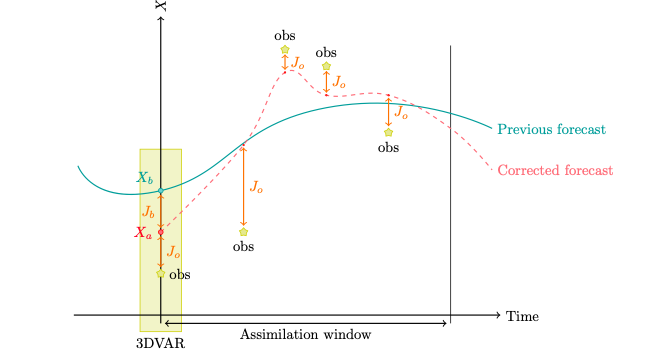
\includegraphics[width=0.8\textwidth]{"images/schema_3D_Var.png"}
	\end{center}
\subsubsection{From 3DVar to BLUE}
\noindent We have are 3D-Var cost function:
$$J(x)=\frac{1}{2}\|x-x^b\|_B^2+\frac{1}{2}\|H(x)-y\|_{R}^2 $$
 Let us minimize J and compute the variation of $J(x)$ with respect to
a variation of $x$ :
$$\begin{aligned}
\delta J(x)=&\frac{1}{2}(\delta x)^TB^{-1}(x-x^b) \\
&+\frac{1}{2}(x-x^b)^TB^{-1}\delta x \\ &+\frac{1}{2}(-H(\delta x))^TR^{-1}(y-H(x)) \\
&+\frac{1}{2}(x^b-H(x))R^{-1}(-H(\delta x)) \\
=&(\delta x)^TB^{-1}(x-x^b)-(\delta x)^TH^TR^{-1}(y-H(x)) \\
=&(\delta x)^T \nabla J
\end{aligned}$$
The extremum condition is 
$$\nabla J=B^{-1}(x^*-x^b)-H^TR^{-1}(y-Hx^*)=0$$
so we will have:
$$x^*=x^b+(B^{-1}+H^TR^{-1}H)^{-1}H^TR^{-1}(y-Hx^b)$$
Grave to Sherman-Morrison-Woodbury identity,
$$K^*=(B^{-1}+H^TR^{-1}H)^{-1}H^TR^{-1}=BH^T(R+HBH^T)^{-1}$$
Therefore, we have that our solution $x$ of the minimization problem coincides with the BLUE optimal analysis $x^a$
\subsection{Ensemble Kalman Filter}
\noindent We have seen so far two methods to do data assimilation, these methods are valid only for linear systems, but the Lorenz system is non-linear, that's why we will introduce the Ensemble Kalman Filter method which works well for non-linear systems. The ENKF method consists in using the Kalman filter method in high dimension and replace P by a set of states $x_1,x_2,..,x_{m}$. So we can approximate the moments of the error by the moments of the sample.
The we have:
$$x_i^a=x_i^f+K[y-h(x_i^f)]$$
We can also define the Kalman gains: 
$$K=P^f H^T(HP^f H^T+R)^{-1}$$
To begin with we can estimate the
forecast error covariance matrix as:
$$P^f=\frac{1}{m-1}\sum_{i=1}^{m}(x_i^f-\bar{x}^f)(x_i^f-\bar{x}^f)^T~~with~~\bar{x}^f=\frac{1}{m}\sum_{i=1}^{m}x_i^f $$ 
We can factorized the forecast error covariance matrix by:
$$P^f=X_f X_f^T$$
where $X_f$ is an $n \times m$ matrix whose columns are the normalized anomalies or normalized perturbations,
$$[X_f]_i=\frac{x_i^f-\bar{x}^f}{\sqrt{m-1}}$$
In addition, we have:
$$
\bar{x}^a=\frac{1}{m}\sum_{i=1}^mx_i^a~~,~~~~[X_a]_i=\frac{x_i^a-\bar{x}^a}{\sqrt{m-1}} $$